%%%%%%%%%%%%%%%%%%%%%%%%%%%%%%%%%%%%%%%%%%%%%%%%%%%%%%%%%%%%%%%%

% IEEEconf.cls file must exist in the same directory as the TeX file you want to compile
\documentclass[letterpaper, 10 pt, conference]{IEEEconf}

\title{\LARGE \bf
Computer History:\\Integrated Circuits
}
%why is the first email the only one that is small?
\author{Jordan Medina\\Kenji Helms\\Guillmer Germino\\
\small guillmer.germino@student.nmt.edu\\
\small kenji.helms@student.nmt.edu\\
\small jordan.medina@student.nmt.edu\\
\small {October 2020}
}

% Image/graphics support
\usepackage{graphicx} % takes care of graphic
\graphicspath{ {./images/} } %full file path to the images

% Formatting for lists
\usepackage{enumitem}

% Formatting for media
\usepackage{float}
\restylefloat{table}
\restylefloat{figure}
\usepackage[utf8]{inputenc}
\usepackage{epigraph}
\usepackage{graphicx}
\usepackage{caption}

\begin{document}


\maketitle

%%%%%%%%%%%%%%%%%%%%%%%%%%%%%%%%%%%%%%%%%%%%%%%%%%%%%%%%%%%%%%%%%%%%%%%%%%%%%%%%
\section{\underline{Introduction}\\\\
\small {\underline{The Confluence of Hardware and Software}}}
%maybe write more about how abstract processes are carried out by physical circuitry/ logical gates
The road from logic to physical computational devices winds through mechanical engineering, electrodynamics, and pure mathematics. The most fundamental mathematical operations within basic logic can be translated to an arbitrary number of physical forms of nearly any  variety. Utility, however, lies in discovering how to reliably produce user-friendly, stable forms for carrying out such tasks. Integrated Circuits, devices at the heart of modern electronic computation, stand at the pinnacle of this technological challenge, and combine size, efficiency, and raw computational power. Though, in essence, they perform the same fundamental tasks of the most rudimentary forms of logical processors, integrated circuits represent a mastery over physical obstacles which allow the blisteringly rapid speed of modern digital life.


\section{History}
\subsection{Ambitious Beginnings}

As early as 1842, the vast potential of computation was known to the prescient minds of Augusta Ada and Charles Babbage. After working on his Difference Engine, Babbage's Analytical Engine took on the task of performing programmable calculations. With the careful help of Ada (commonly known as Ada Lovelace), the Analytical Engine was designed to: receive punch cards for initiating user input, store memory within the state of its mechanical wheels, perform the calculation of arithmetic operation, and return output in the form of punch cards and bells rings. 

\begin{figure}[h!]
\centering
\captionsetup{justification=centering}
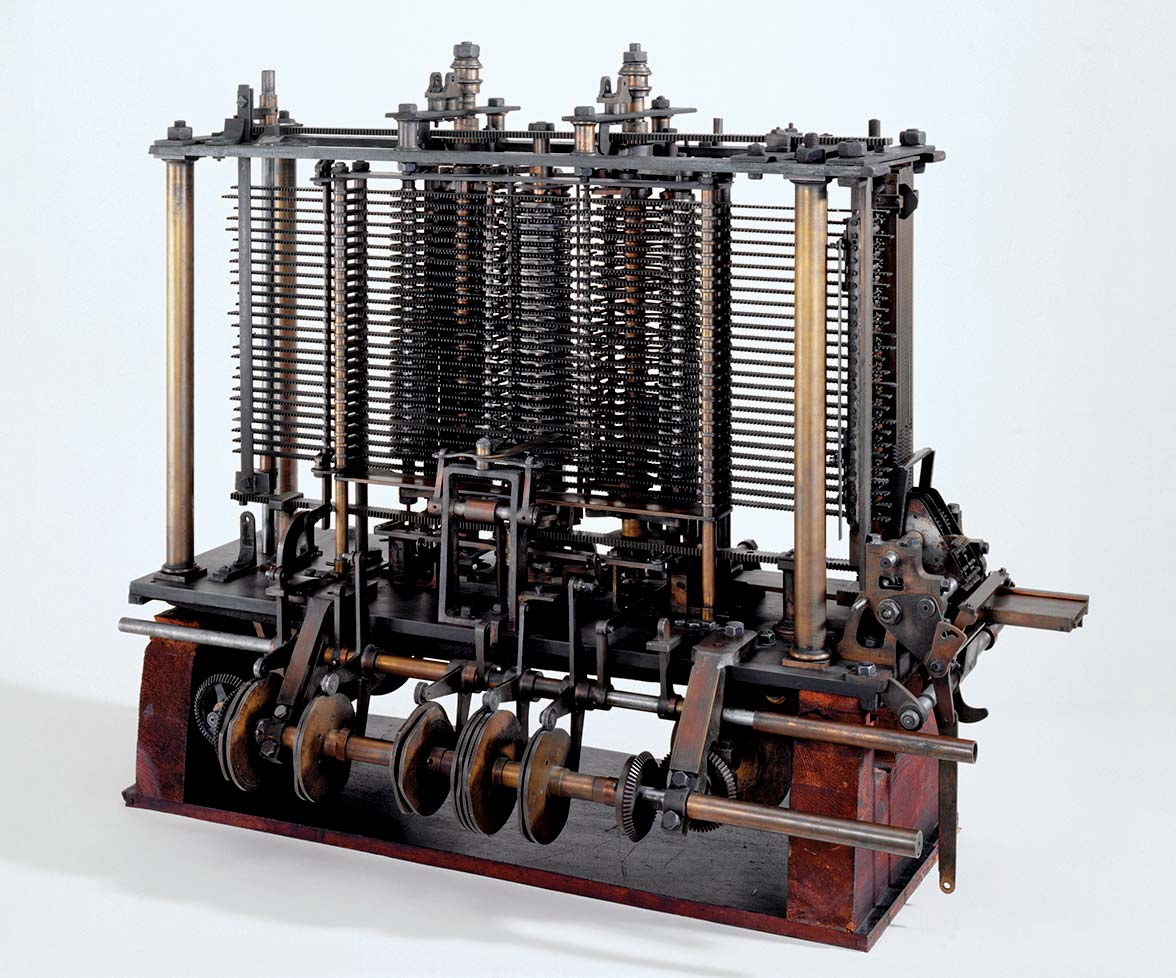
\includegraphics[width=0.2\textwidth]{portion-Charles-Babbage-Analytical-Engine-death-mill-1871.jpg}
\caption{The first general purpose computer, the Analytical Engine}
\label{fig:example}
\end{figure} 

In this form of the "computer", it is the relatively large components of mechanical gears and pegs which instantiate the logic of the underlying mathematics. Without a hint of modern electronic technology, logically meaningful instruction was stored in the macroscopic states of the wheels, which allow for the processing of input to output via mathematical rules. This incredible device was unfortunately left unfinished, but its design proved to be Turing-complete, essentially deeming the Analytic Engine as a true computer, an astonishing achievement for Victorian Age technology. 

\subsection{Vacuum Tube Technology}
With the prevalence of electricity-driven technology 

\begin{figure}[h!]
\centering
\captionsetup{justification=centering}
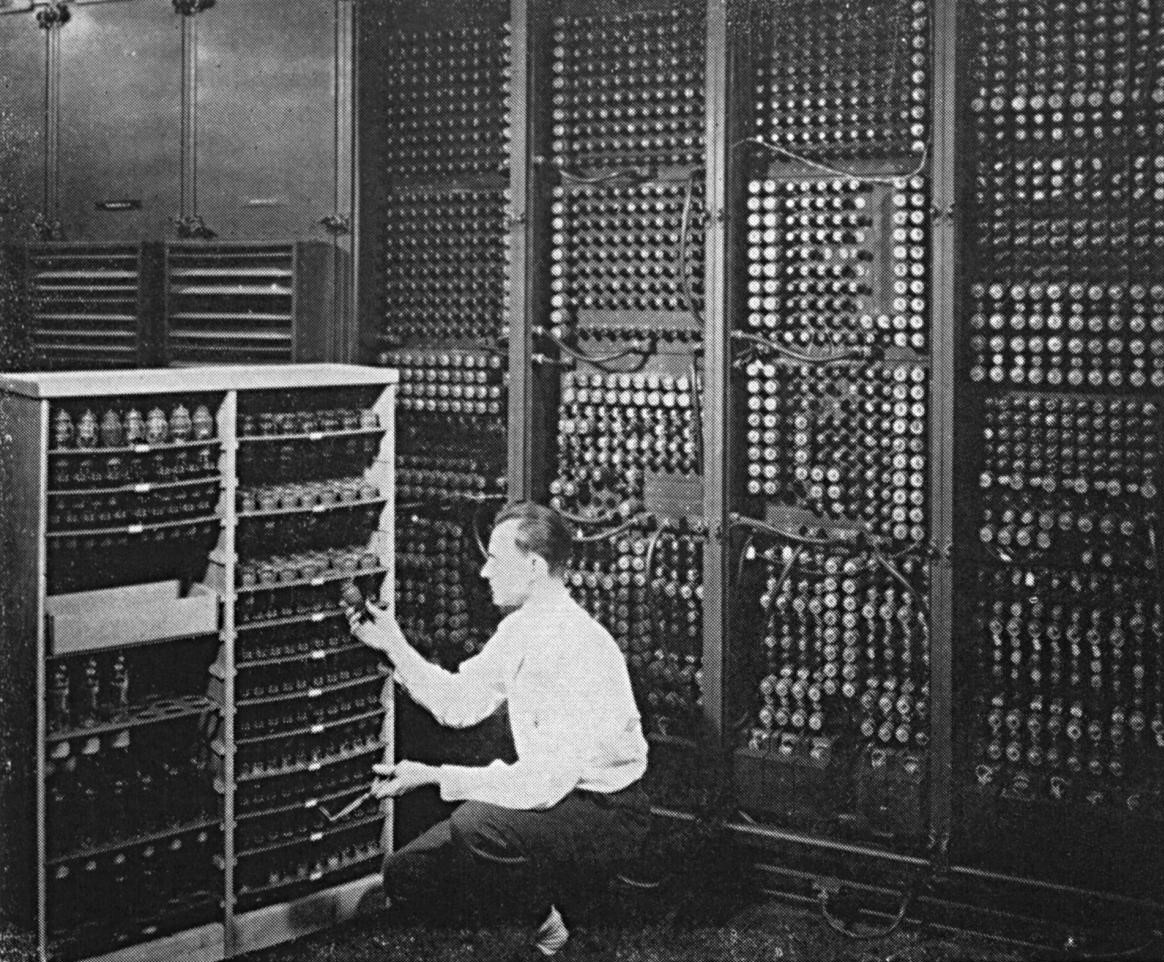
\includegraphics[width=0.2\textwidth]{ENIAC-changing_a_tube.jpg}
\caption{A technician changes a vacuum tube in the ENIAC}
\label{fig:example}
\end{figure} 



%Talk about the timeline from vacuum tube, 

\section{Theory}

Talk about the necessity of using circuits. Why are they needed at all? How do they accomplish the basic ideas from a model of information transfer/logic?


\section{Moore's Law}


\begin{figure}[h!]
\centering
\captionsetup{justification=centering}
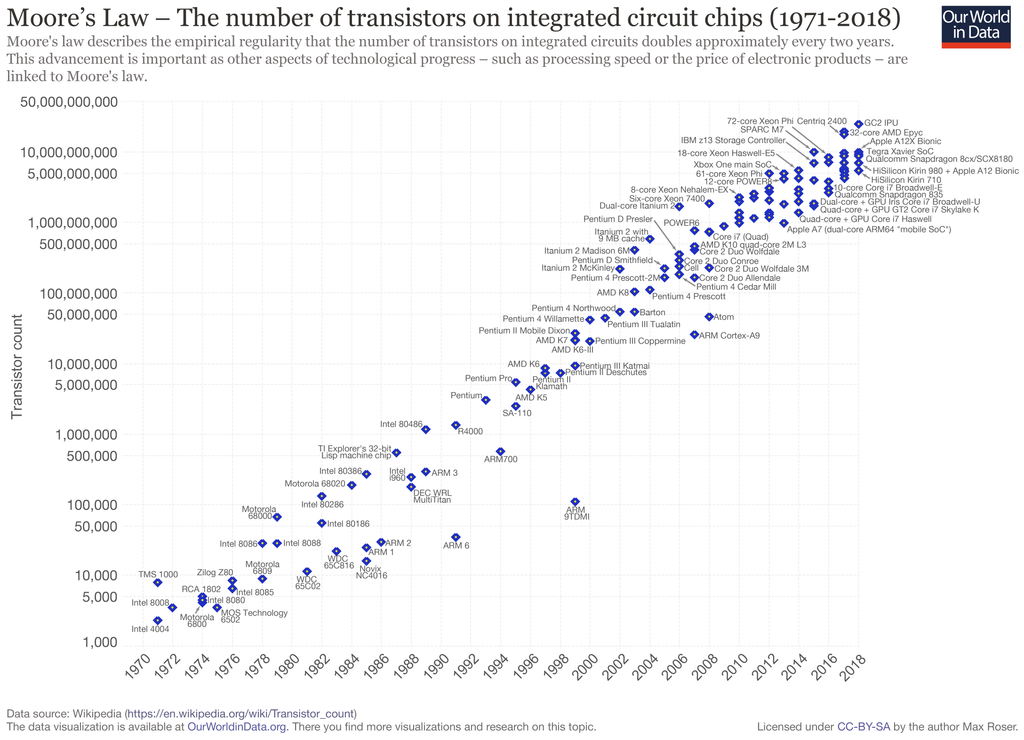
\includegraphics[width=0.2\textwidth]{1024px-Moore's_Law_Transistor_Count_1971-2018.png}
\caption{Integrated Circuit complexity over time, 1970-2018}
\label{fig:example}
\end{figure} 
Integrated Circuits have gone through an immense growth per physical size over the years, leading to many of the breakthroughs enjoyed in modern technology. Talk about how Moore's Law uses ICs as a metric of computer tech sophistication.


\section{Cost/Efficiency}



\section{CONCLUSION}

Conclude the ideas.

\section*{REFERENCES}


\begin{enumerate}[label={[\arabic*]}]
\item https://www.newegg.com/p/N82E16811112392
\item https://www.nvidia.com/en-us/geforce/graphics-cards/30-series/rtx-3080/
\item https://www.intel.com/content/www/us/en/products/processors/core/i9-processors/i9-10900.html
\item https://www.newegg.com/corsair-32gb-260-pin-ddr4-so-dimm/p/N82E16820236682
\item https://www.pcmag.com/reviews/acer-predator-x27
\item https://www.amazon.com/Toshiba-Performance-Desktop-Internal-HDWE150XZSTA/dp/B013JPLKQK
\end{enumerate}

\end{document}


